\clearpage

\section{Opaque without Survivability - Reference Network} \label{Reference_Network}

In this case study we focus on the opaque case without survivability for the reference network.
The opaque transport mode performs OEO (optical-electric-optical) conversions on each intermediate node from the source to the destination node.
One advantage of this mode of transport is that it eliminates accumulation of physical impairments, and allows optimum grooming by performing grooming at each node.

\subsection{Physical Network Topology}\label{Reference_Network_Topology}
\begin{tcolorbox}	
\begin{tabular}{p{2.75cm} p{0.2cm} p{10.5cm}} 	
\textbf{Student Name}  &:& Tiago Esteves    (October 03, 2017 - )\\
\end{tabular}
\end{tcolorbox}


In the figure below we ca see that our reference network consists of 6 nodes and 8 Bidirectional links.
The average length of the links was chosen so that the following calculations are more simplistic, for this was created a matrix of distances between the respective nodes.
Finally, ODU's matrices were also created to be able to determine the total traffic used in each scenario.\\

\begin{figure}[h!]
\centering
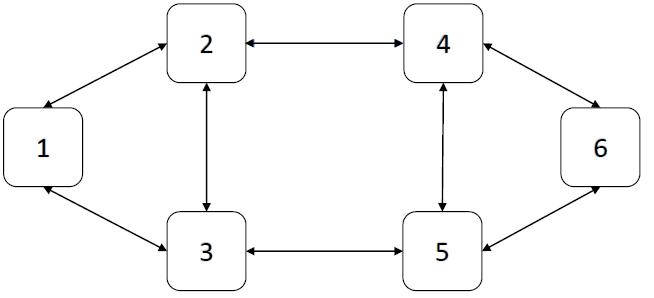
\includegraphics[width=\textwidth]{sdf/opaque/figures/RedeTeste}
\caption{Physical topology of the reference network.}
\end{figure}

\vspace{11pt}
The distance matrix is the same for the two scenarios but the ODU's matrices are not.
In this way only the matrices for the case of low traffic are elucidated, being that in the case of a high traffic it is only necessary to multiply these matrices by the value 10.\\

\[
Dist=
  \begin{bmatrix}
    0 & 500 & 500 & 0 & 0 & 0 \\
    500 & 0 & 400 & 500 & 0 & 0 \\
    500 & 400 & 0 & 0 & 500 & 0 \\
    0 & 500 & 0 & 0 & 600 & 450 \\
    0 & 0 & 500 & 600 & 0 & 550 \\
    0 & 0 & 0 & 450 & 550 & 0
  \end{bmatrix}
\]

\[
ODU0=
  \begin{bmatrix}
    0 & 5 & 1 & 3 & 1 & 3 \\
    5 & 0 & 0 & 1 & 5 & 0 \\
    1 & 0 & 0 & 1 & 4 & 1 \\
    3 & 1 & 1 & 0 & 1 & 0 \\
    1 & 5 & 4 & 1 & 0 & 3 \\
    3 & 0 & 1 & 1 & 3 & 0
  \end{bmatrix}
\quad ODU1=
  \begin{bmatrix}
    0 & 2 & 4 & 2 & 0 & 5 \\
    2 & 0 & 0 & 3 & 1 & 1 \\
    4 & 0 & 0 & 1 & 1 & 0 \\
    3 & 3 & 1 & 0 & 1 & 3 \\
    0 & 1 & 1 & 1 & 0 & 1 \\
    5 & 1 & 0 & 3 & 1 & 0
  \end{bmatrix}
\quad ODU2=
  \begin{bmatrix}
    0 & 1 & 1 & 1 & 0 & 0 \\
    1 & 0 & 0 & 0 & 1 & 0 \\
    1 & 0 & 0 & 1 & 1 & 0 \\
    1 & 0 & 1 & 0 & 1 & 0 \\
    0 & 1 & 1 & 1 & 0 & 1 \\
    0 & 0 & 0 & 0 & 1 & 0
  \end{bmatrix}
\]
\[
ODU3=
  \begin{bmatrix}
    0 & 0 & 0 & 0 & 0 & 0 \\
    0 & 0 & 1 & 0 & 0 & 1 \\
    0 & 1 & 0 & 0 & 1 & 0 \\
    0 & 0 & 0 & 0 & 0 & 0 \\
    0 & 0 & 1 & 0 & 0 & 0 \\
    0 & 1 & 0 & 0 & 0 & 0
  \end{bmatrix}
\qquad ODU4=
  \begin{bmatrix}
    0 & 0 & 0 & 0 & 0 & 0 \\
    0 & 0 & 0 & 0 & 0 & 1 \\
    0 & 0 & 0 & 0 & 0 & 0 \\
    0 & 0 & 0 & 0 & 0 & 0 \\
    0 & 0 & 0 & 0 & 0 & 1 \\
    0 & 1 & 0 & 0 & 1 & 0
  \end{bmatrix}
\]

\vspace{17pt}

The values indicated in the distance matrix, referred to below, are expressed in kilometers (Km) and as it couldn't be otherwise, this matrix is symmetric.
In relation to the traffic matrices each ODU, referred previously, has its respective value being that the ODU0 corresponds to 1.25 Gbits/s, ODU1 to 2.5 Gbits/s, ODU2 to 10 Gbits/s, ODU3 to 40 Gbits/s and finally the ODU4 corresponds to 100 Gbits/s.
As we can see these matrices are bidirectional because they are symmetric matrices and as such the traffic sent in one direction must be the same traffic sent in the opposite direction. \\

Through these ODU's we can calculate total network traffic for the low traffic scenario:\\

$T_1^0$ = 60x1.25 = 75 Gbits/s \qquad
$T_1^1$ = 50x2.5 = 125 Gbits/s \qquad
$T_1^2$ = 16x10 = 160 Gbits/s \\

$T_1^3$ = 6x40 = 240 Gbits/s \quad
$T_1^4$ = 4x100 = 400 Gbits/s \\

$T_{1}$ = 75 + 125 + 160 + 240 + 400 = 1000 Gbits/s \qquad
$T$ = 1000/2 = 0.5 Tbits/s\\

Where the variable $T_1^x$ represents the unidirectional traffic of the ODUx, for example, $T_1^0$ represents the unidirectional traffic of the ODU0 and $T_1^1$ represents the unidirectional traffic of the ODU1. The variable $T_{1}$ represents the total of unidirectional traffic that is injected into the network and finally the variable $T$ represents the total of bidirectional traffic.\\

We can thus conclude that the total traffic for the two scenarios is as follows:
\begin{itemize}
  \item Low Traffic: \textbf{0.5 TBits/s}
  \item High Traffic: \textbf{5 TBits/s}
\end{itemize}

Finally for this project has to take into consideration the table \ref{table_ref_net} because in it we can see the values of the variables associated with this network.
\begin{table}[h!]
\centering
\begin{tabular}{|| c | c | c||}
 \hline
 Constant & Description & Value \\
 \hline\hline
 N & Number of nodes & 6 \\
 L & Number of bidirectional links & 8 \\
 <$\delta$> & Node out-degree & 2.667 \\
 <len> & Mean link length (km) & 500 \\
 <h> & Mean number of hops for working paths & 1.533 \\
 <h'> & Mean number of hops for backup paths & 2.467 \\
 \hline
\end{tabular}
\caption{Table of reference network values}
\label{table_ref_net}
\end{table}

\subsection{Dimensioning using Analytical Model}
\begin{tcolorbox}	
\begin{tabular}{p{2.75cm} p{0.2cm} p{10.5cm}} 	
\textbf{Student Name}  &:& Tiago Esteves    (October 03, 2017 - )\\
\end{tabular}
\end{tcolorbox}

In this section we will do the dimensioning of the network mentioned in the previous subsection to calculate the value of your CAPEX, for this we will use the analytical formulations so as to obtain the best solution but for this we will also have to take into account the cost of the equipment used that can be consulted in table \ref{table_cost_opaque}.
First will be mentioned all the formulas and calculations needed for the CAPEX of the network. Next will be described the calculations and the results obtained for this network.\\

\begin{table}[h!]
\centering
\begin{tabular}{|| c | c||}
 \hline
 Equipment & Cost \\
 \hline\hline
 OLT without transponders & 15000 \euro \\
 Transponder & 5000 \euro/Gb \\
 Optical Amplifier & 4000 \euro \\
 EXC & 10000 \euro \\
 OXC & 20000 \euro \\
 EXC Port & 1000 \euro /Gb/s\\
 OXC Port & 2500 \euro /porto \\
 \hline
\end{tabular}
\caption{Table with costs}
\label{table_cost_opaque}
\end{table}


\subsubsection{Analytical Equations}

To know the value of CAPEX it is necessary to know the value of the cost of the links and the cost of the nodes.
To calculate the cost of the Links we will use the equation \ref{analytical_linkCosts}

\begin{equation}
C_L = \left(2 \times L \times \gamma_0^{OLT}\right) + \left(2 \times L \times \gamma_1^{OLT} \times \tau \times <w>\right) + \left(N^R \times c^R\right)
\label{analytical_linkCosts}
\end{equation}

\begin{itemize}
\item{$C_L$				$\rightarrow$	Links cost}
\item{$\gamma_0^{OLT}$	$\rightarrow$	OLT cost in euros}
\item{$L$				$\rightarrow$	Number of unidirectional links}
\item{$\gamma_1^{OLT}$	$\rightarrow$	Transponder cost in euros}
\item{$<w>$             $\rightarrow$   Average number of optical channels}
\item{$\tau$		    $\rightarrow$	Traffic per port}
\item{$N^R$				$\rightarrow$	Total number of optical amplifiers}
\item{$c^R$				$\rightarrow$	Optical amplifiers cost in euros}
\end{itemize}


To calculate the cost of the nodes, the sum of the costs of the optical and electrical node is made. For this case the value of the optical cost is zero only needing to know the electric cost of the nodes that is given by equation \ref{analytical_electricalCost}

\begin{equation}
C_{exc} = N \times \left( \gamma_{e0} + \left( \gamma_{e1} \times \tau \times <P_{exc}> \right) \right)
\label{analytical_electricalCost}
\end{equation}

\begin{itemize}
\item{$C_{exc}$		$\rightarrow$	Electrical ports cost}
\item{$N$			$\rightarrow$	Number of nodes}
\item{$\gamma_{e0}$	$\rightarrow$	EXC cost in euros}
\item{$\gamma_{e1}$	$\rightarrow$	EXC port cost in euros}
\item{$\tau$		$\rightarrow$	Traffic per port}
\item{$<P_{exc}>$   $\rightarrow$   Average number of ports of the electrical switch}
\end{itemize}


Looking at the equation \ref{analytical_linkCosts} we can see that we already have practically all the values of the variables used. Assuming that $\tau$ is 100 Gbits/s is thus only missing the number of optical amplifiers and the number of optical channels where they can be calculated by equation \ref{amplifiers} and \ref{optical_channels} respectively.\\

\begin{equation}
N^R = \sum\limits_{l=1}^L\left(\left\lceil\frac{len_l}{span}\right\rceil-1\right)
\label{amplifiers}
\end{equation}

\begin{itemize}
\item{$N^R$			$\rightarrow$ Total number of regenerators/amplifiers}
\item{$len_l$		$\rightarrow$ Length of link l}
\item{$span$		$\rightarrow$ Distance between amplifiers}	
\end{itemize}	

\begin{equation}
<w> = \left( \frac{\lceil D \times <h> \rceil}{L} \right) \times \left( 1 + <k>\right)
\label{optical_channels}
\end{equation}

\begin{itemize}
\item{$<w>$		$\rightarrow$ Average number of optical channels}
\item{$D$  		$\rightarrow$ Number of bidirectional demands}
\item{$L$		$\rightarrow$ Number of Links}	
\item{$<k>$		$\rightarrow$ Survivability coefficient}
\end{itemize}	

where:
\begin{equation}
D = \left(\frac{1}{2}\right) \times \left( 1 + \xi \right) \times \left(\frac{T_1}{\tau}\right)
\label{demands}
\end{equation}

\begin{itemize}
\item{$D$  		$\rightarrow$ Number of bidirectional demands}
\item{$\xi$		$\rightarrow$ xxxxxxxxxxx}
\item{$T_1$		$\rightarrow$ Total unidirectional traffic}	
\item{$\tau$	$\rightarrow$ Traffic per port}
\end{itemize}


Finally looking at the equation \ref{analytical_electricalCost} we can see that we already have practically all the values with the exception of the number of ports the electrical switch that can be calculated through the equation \ref{Pexc_opaque}

\begin{equation}
<P_{exc}> = <d> \times [1 + \left(1 + <k>\right) \times <h>]
\label{Pexc_opaque}
\end{equation}

\begin{itemize}
\item{$<P_{exc}>$ $\rightarrow$ Average number of ports of the electrical switch}
\item{$<d>$		  $\rightarrow$ Average number of demands}
\item{$<k>$		  $\rightarrow$ Survivability coefficient}	
\item{$<h>$	      $\rightarrow$ Average number of hops}
\end{itemize}

Where:
\begin{equation}
<d> = \frac{2 \times D}{N}
\label{average_demand}
\end{equation}

\subsubsection{Results}

We already have all the necessary formulas to obtain the CAPEX value for this specific network. As described in the subsection of the network topology we have two values of network traffic, low traffic and high traffic, soon we will get two different CAPEX. Finally we have to take into account that as it is the opaque transport mode, the value of $\xi$ is 1 and because it is without survivability, the value of $<k>$ is 0. Then we can rewrite the equations.\\

\textbf{Scenario 1: Reference Network Low Traffic}\\

Using equation \ref{demands}:\\

$D$ = $\frac{1}{2}$ * $($ 1 + 1 $)$ * $($ $\frac{1000}{100}$ $)$ \qquad \qquad $D$ = 10\\

Replacing in equation \ref{optical_channels}:\\

$<w>$ = $($ $\frac{10 * 1.533}{8}$ $)$ * $($ 1 + 0$)$ \qquad \qquad $<w>$ = 2\\

Using equation \ref{amplifiers}:\\

$N^R$ = $($ $\frac{500}{100}$-1 $)$ + $($ $\frac{500}{100}$-1$)$ + $($ $\frac{400}{100}$-1 $)$ + $($ $\frac{500}{100}$ -1$)$ + $($ $\frac{500}{100}$-1$)$ + $($ $\frac{600}{100}$-1$)$ + $($ $\frac{450}{100}$-1$)$ + $($ $\frac{550}{100}$-1$)$\\

$N^R$ = 33\\

Finally, replacing all in equation \ref{analytical_linkCosts} the Link Cost is:\\

$C_L$ = $($2 * 8 * 15000$)$ + $($2 * 8 * 5000 * 100 * 2$)$ + $($33 * 4000$)$\\

$C_L$ = \textbf{16 372 000 \euro}\\

In relation to the cost of the nodes we first use the equation \ref{average_demand}:\\

$<d>$ = $\frac{2 * 10}{6}$ \qquad \qquad $<d>$ = 3.333\\

Replacing in equation \ref{Pexc_opaque}:\\

$<P_{exc}>$ = 3.333 * $[$1 + $($1 + $0$ $)$ * 1.533$]$ \qquad \quad $<P_{exc}>$ = 8.4425 \\

Finally, replacing all in equation \ref{analytical_electricalCost} the Node Cost is:\\

$C_N$ = $C_{exc}$ = 6 * $($10000 + $($1000 * 100 * 8.4425 $)$ $)$\\

$C_N$ = \textbf{5 125 500 \euro}\\

The CAPEX is:\\
$CAPEX$ = 16 372 000 + 5 125 500\\

$CAPEX$ = \textbf{21 497 500 \euro}\\

\textbf{Scenario 2: Reference Network High Traffic}\\

Using equation \ref{demands}:\\

$D$ = $\frac{1}{2}$ * $($ 1 + 1 $)$ * $($ $\frac{1000}{100}$ $)$ \qquad \qquad $D$ = 100\\

replacing in equation \ref{optical_channels}:\\

$<w>$ = $($ $\frac{100 * 1.533}{8}$ $)$ * $($ 1 + 0$)$ \qquad \quad $<w>$ = 20\\

Finally, replacing all in equation \ref{analytical_linkCosts} the Link Cost is:\\

$C_L$ = $($2 * 8 * 15000$)$ + $($2 * 8 * 5000 * 100 * 20$)$ + $($33 * 4000$)$\\

$C_L$ = \textbf{160 372 000 \euro}\\

In relation to the cost of the nodes we first use the equation \ref{average_demand}:\\

$<d>$ = $\frac{2 * 100}{6}$ \qquad \qquad $<d>$ = 33.333\\

Replacing in equation \ref{Pexc_opaque}:\\

$<P_{exc}>$ = 33.333 * $[$1 + $($1 + $0$ $)$ * 1.533$]$ \qquad \qquad $<P_{exc}>$ = 84.4325 \\

Finally, replacing all in equation \ref{analytical_electricalCost} the Node Cost is:\\

$C_N$ = $C_{exc}$ = 6 * $($10000 + $($1000 * 100 * 84.4325 $)$ $)$\\

$C_N$ = \textbf{8 453 250 \euro}\\

The CAPEX is:\\
$CAPEX$ = 160 372 000 + 8 453 250\\

$CAPEX$ = \textbf{168 825 250 \euro}\\


\subsection{Dimensioning using ILP}
\begin{tcolorbox}	
\begin{tabular}{p{2.75cm} p{0.2cm} p{10.5cm}} 	
\textbf{Student Name}  &:& Tiago Esteves    (October 03, 2017 - )\\
\end{tabular}
\end{tcolorbox}

\vspace{11pt}
In this section we will do the dimensioning of the network mentioned in the first subsection to calculate the value of your CAPEX, for this we will use the ILP model describe in section \ref{ILP_Opaque_Survivability} and we can get the best possible solution.
In the initial subsection will be described the network cost where all the formulas and calculations necessary to obtain the CAPEX of the network will be mentioned.
Finally, in the last subsection, the results obtained through the described model will be presented.

\subsubsection{Network costs}\label{Net_Costs}

In this phase the results will be presented to calculate the CAPEX of the reference network.
The value of the CAPEX of the network will be calculated based on the costs of the equipment present in the table \ref{table_cost_opaque}.
In addition to the equipment costs we will also use the parameter "span", which in this case will have a value of 100, because this value is used to calculate the number of optical amplifiers required in the network using Equation \ref{amplifiers}.\\

To know the value of CAPEX it is necessary to know the value of the cost of the links and the cost of the nodes.
To calculate the cost of the nodes, the sum of the costs of the optical and electrical node is made. For this case the value of the optical cost is zero only needing to know the electric cost of the nodes that is given by equation \ref{electricalCostOpaque}.

\begin{equation}
C_{exc} = \left(\gamma_{e0}\times N\right) + \gamma_{e1} \times \left(T_1 + \left(2 \times w^0 \times \tau \right)\right)
\label{electricalCostOpaque}
\end{equation}

\begin{itemize}
\item{$C_{exc}$		$\rightarrow$	Electrical ports cost}
\item{$\gamma_{e0}$	$\rightarrow$	EXC cost in euros}
\item{$N$			$\rightarrow$	Number of nodes}
\item{$\gamma_{e1}$	$\rightarrow$	EXC port cost in euros}
\item{$T_1$         $\rightarrow$   Total unidirectional traffic}
\item{$w^0$			$\rightarrow$	Total number of optical channels}
\item{$\tau$		$\rightarrow$	Traffic per port}
\end{itemize}

\vspace{11pt}

To calculate the cost of the Links we will use the equation \ref{linkCosts}.

\begin{equation}
C_L = \left(2 \times \gamma_0^{OLT} \times L\right) + \left(2 \times \gamma_1^{OLT} \times \tau \times W\right) + \left(N^R \times c^R\right)
\label{linkCosts}
\end{equation}	
	
\begin{itemize}
\item{$C_L$				$\rightarrow$	Links cost}
\item{$\gamma_0^{OLT}$	$\rightarrow$	OLT cost in euros}
\item{$L$				$\rightarrow$	Number of unidirectional links}
\item{$\gamma_1^{OLT}$	$\rightarrow$	Transponder cost in euros}
\item{$W$             $\rightarrow$	    Total number of optical channels}
\item{$N^R$				$\rightarrow$	Total number of optical amplifiers}
\item{$c^R$				$\rightarrow$	Optical amplifiers cost in euros}
\end{itemize}

\subsubsection{ILP Results}

To perform the calculations using the implementation of the models described in section \ref{ILP_Opaque_Survivability} it is necessary to use a mathematical software tool. For this we will use MATLAB which is ideal for dealing with linear programming problems and can call the LPsolve through an external interface. \\

\textbf{Scenario 1: Reference Network Low Traffic} \label{Scenario1_opaque} \\

In this scenario we used the table \ref{table_ref_net}. In the table \ref{result_ILP1_reference} we can see the values calculated through MatLab and using the values indicated in table \ref{table_cost_opaque} we can finally calculate the CAPEX value.
\begin{table}[h!]
\centering
\begin{tabular}{|| c | c||}
 \hline
 Number of optical channels & Value \\
 \hline\hline
 in the link (1,2) & 1 \\
 in the link (1,3) & 1 \\
 in the link (2,3) & 1 \\
 in the link (2,4) & 2 \\
 in the link (3,5) & 1 \\
 in the link (4,5) & 1 \\
 in the link (4,6) & 2 \\
 in the link (5,6) & 2 \\
 \hline
\end{tabular}
\caption{Table with results}
\label{result_ILP1_reference}
\end{table}

Using equation \ref{linkCosts} : \\
$C_L$ = $($2 * 15 000 * 8$)$ + $($2 * 5 000 * 100 * 11$)$ + $($33 * 4 000$)$ \\
$C_L$ = \textbf{11 372 000 \euro} \\


Using equation \ref{electricalCostOpaque} : \\
$C_{exc}$ = $($6 * 10 000$)$ + 1 000 * $($1 000 + $($2 * 11 * 100$)$ $)$ \\
$C_N$ = $C_{exc}$ = \textbf{3 260 000 \euro} \\

$CAPEX$ = 11 372 000 + 3 260 000 \\
$CAPEX$ = \textbf{14 632 000 \euro}\\

Through image \ref{scriptopaque_surv_ref_low} we can see that the previous ILP based calculations are correct.
\begin{figure}[h!]
\centering
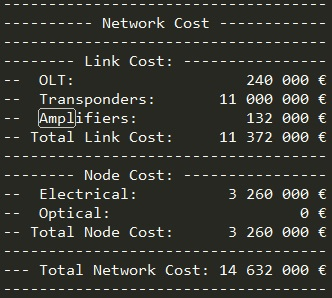
\includegraphics[width=8cm]{sdf/opaque/figures/script_opaque_surv_ref_low}
\caption{The ILP script used with the network cost.}
\label{scriptopaque_surv_ref_low}
\end{figure}


\textbf{Scenario 2: Reference Network High Traffic} \label{Scenario2_opaque} \\

In this scenario we used again the table \ref{table_ref_net}. In the table \ref{result_ILP2_reference} we can see the values calculated through MatLab and using the values indicated in table \ref{table_cost_opaque} we can finally calculate the CAPEX value.
\begin{table}[h!]
\centering
\begin{tabular}{|| c | c||}
 \hline
 Number of optical channels & Value \\
 \hline\hline
 in the link (1,2) & 4 \\
 in the link (1,3) & 4 \\
 in the link (2,3) & 4 \\
 in the link (2,4) & 19 \\
 in the link (3,5) & 9 \\
 in the link (4,5) & 5 \\
 in the link (4,6) & 16 \\
 in the link (5,6) & 14 \\
 \hline
\end{tabular}
\caption{Table with results}
\label{result_ILP2_reference}
\end{table}

Using equation \ref{linkCosts} : \\
$C_L$ = $($2 * 15 000 * 8$)$ + $($2 * 5 000 * 100 * 75 $)$ + $($33 * 4 000$)$ \\
$C_L$ = \textbf{ 75 372 000 \euro} \\

Using equation \ref{electricalCostOpaque} : \\
$C_{exc}$ = $($6 * 10 000$)$ + 1 000 * $($10 000 + $($2 * 75 * 100$)$ $)$ \\
$C_N$ = $C_{exc}$ = \textbf{25 060 000 \euro} \\

$CAPEX$ = 75 372 000 + 25 060 000 \\
$CAPEX$ = \textbf{100 432 000 \euro}\\

Through image \ref{scriptopaque_surv_ref_high} we can see that the previous ILP based calculations are correct.
\begin{figure}[h!]
\centering
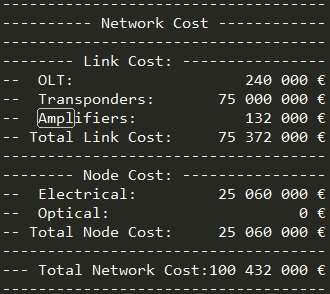
\includegraphics[width=8cm]{sdf/opaque/figures/script_opaque_surv_ref_high}
\caption{The ILP script used with the network cost.}
\label{scriptopaque_surv_ref_high}
\end{figure}


\subsection{Dimensioning using Heuristics}
\begin{tcolorbox}	
\begin{tabular}{p{2.75cm} p{0.2cm} p{10.5cm}} 	
\textbf{Student Name}  &:& Tiago Esteves    (October 03, 2017 - )\\
\end{tabular}
\end{tcolorbox}

\vspace{11pt}
In this section we will, again, do the dimensioning of the network mentioned in the first subsection to calculate the value of your CAPEX, for this we will use the Heuristic model describe in section \ref{heuristic_Opaque_Survivability} and we can get the best possible solution.
The software used to implement the above heuristics is Net2Plan.
In an initial phase will be described in a simple way how net2plan works, if a more complete description is necessary we can always consult the appendice \ref{net2planguide}, next will be presented the results for the scenarios mentioned previously.

\subsubsection{Net2Plan description}

In an initial phase we will have two aspects to fulfill. The first one is to define the ODU0, ODU1, ODU2, ODU3 and ODU4 matrices, and the second one passes through the design of the network in question.
After this phase is completed, we then apply the algorithms created. first the "joinTrafficMatrices" then the "logicalTopology" and finally the "Grooming".
At the end, the algorithm "CostReport" will be applied to obtain the CAPEX result for the network in question.

\subsubsection{Heuristics Results}

\textbf{Scenario 1: Reference Network Low Traffic}\\

Following all the steps mentioned in the previous subsection and using all the data referring to this scenario the obtained result can be consulted in the following table \ref{heuristicopaque_surv_ref_low}.

\begin{figure}[h!]
\centering
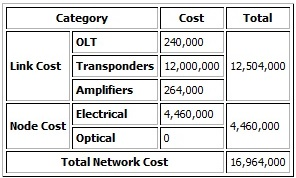
\includegraphics[width=9cm]{sdf/opaque/figures/heuristic_opaque_surv_ref_low}
\caption{The network cost using Net2Plan.}
\label{heuristicopaque_surv_ref_low}
\end{figure}


\textbf{Scenario 2: Reference Network High Traffic}\\

Following all the steps mentioned in the previous subsection and using all the data referring to this scenario the obtained result can be consulted in the following table \ref{heuristicopaque_surv_ref_high}.

\begin{figure}[h!]
\centering
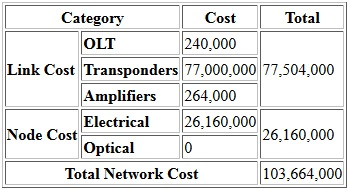
\includegraphics[width=9cm]{sdf/opaque/figures/heuristic_opaque_surv_ref_high}
\caption{The network cost using Net2Plan.}
\label{heuristicopaque_surv_ref_high}
\end{figure}


\subsection{Comparative Analysis}
\begin{tcolorbox}	
\begin{tabular}{p{2.75cm} p{0.2cm} p{10.5cm}} 	
\textbf{Student Name}  &:& Tiago Esteves    (October 03, 2017 - )\\
\end{tabular}
\end{tcolorbox}

\vspace{11pt}
In this subsection we will compare the CAPEX values obtained for the two scenarios in the three types of dimensioning. For a better analysis of the results will be created the table \ref{table_comparative_opaque_sur_ref_1} (scenario 1) and the table \ref{table_comparative_opaque_sur_ref_2} (scenario 2) with the different values obtained.\\

\textbf{Scenario 1:}\\

\begin{table}[h!]
\centering
\begin{tabular}{| c | c | c | c |}
 \hline
   & Analytical & ILP & Heuristic \\
 \hline\hline
 Link Cost & 16 372 000 \euro & 11 372 000 \euro & 12 504 000 \euro \\
 Node Cost & 5 125 500 \euro & 3 260 000 \euro & 4 460 000 \euro \\
 CAPEX & \textbf{21 497 500 \euro} & \textbf{14 632 000 \euro} & \textbf{16 964 000 \euro} \\
 \hline
\end{tabular}
\caption{Table with different value of CAPEX }
\label{table_comparative_opaque_sur_ref_1}
\end{table}

\vspace{11pt}
Looking at the previous table we can make some comparisons between the several different models of dimensioning and finally draw some conclusions.

\begin{itemize}
  \item We can conclude that in this case the dimensioning using ILP is the best (lowest cost).
  \item In comparison with the analytical model we can see that there is a difference considered with a 32\% error, this value is mainly due to the number of optical channels because in the analytical model more optical channels are calculated and used than those required in the ILP model.
  \item In comparison with the heuristic model we can see that there is a small difference with a 14\% error, much smaller than the previous one.
\end{itemize}

\vspace{11pt}
\textbf{Scenario 2:}\\

\begin{table}[h!]
\centering
\begin{tabular}{| c | c | c | c |}
 \hline
   & Analytical & ILP & Heuristic \\
 \hline\hline
 Link Cost & 160 372 000 \euro & 75 372 000 \euro & 77 504 000 \euro \\
 Node Cost & 8 453 250 \euro & 25 060 000 \euro & 26 160 000 \euro \\
 CAPEX & \textbf{168 825 250 \euro} & \textbf{100 432 000 \euro} & \textbf{103 664 000 \euro} \\
 \hline
\end{tabular}
\caption{Table with different value of CAPEX }
\label{table_comparative_opaque_sur_ref_2}
\end{table}

\vspace{11pt}
Looking at the previous table we can make some comparisons between the several different models of dimensioning and finally draw some conclusions.

\begin{itemize}
  \item We can conclude that in this case the dimensioning using ILP is the best (lowest cost).
  \item In comparison with the analytical model we can see that there is a difference considered with a 66\% error.
  \item In comparison with the heuristic model we can see that there is a smaller difference with a 3\% error.
\end{itemize}

